%%%%%%%%%%%%%%%%%%%%%%%%%%%%%%%%%%%%%%%%%%%%%%%%%%%%%%%%%%%%%%%%%%%%%%%%%%%%%%%%%
%
%  Bachelorarbeit Adler Tilman 01.06.2015
%  "Android app for detecting the state of Go games and recording it"
%  Lehrstuhl fuer Mustererkennung, FAU Erlangen-Nuernberg
%
%%%%%%%%%%%%%%%%%%%%%%%%%%%%%%%%%%%%%%%%%%%%%%%%%%%%%%%%%%%%%%%%%%%%%%%%%%%%%%%%%

% ++ LME LateX Dokument
%    Die Verwendung der option "german" bindet german.sty ein.
%    For english papers, use the "english" option and talk to your advisor.
\documentclass[english,bt]{package/lmedoc}
%\documentclass[english,bt]{lmedoc}

\usepackage{hyperref}
\usepackage{graphicx}
\usepackage{subcaption}
\usepackage{sidecap}
\usepackage{multicol}
\usepackage{wrapfig}
\usepackage{tikz}
\usepackage{pgfplots}
\usepackage{multirow}
\usepackage{array}
\usepackage{pgfplotstable}
\input{package/pieChart.tex}
\usepackage{booktabs}
\usepackage{todonotes}

% \usepgfplotslibrary{external}
% \tikzexternalize[prefix=plotcache/]

% ++ Umlaut Unterstuetzung
%    Paket "inputenc" kann verwendet werden, um z.B. Umlaute oder das scharfe S
%    direkt (als Nicht-ASCII-Zeichen) einzubinden. Dabei auf die korrekte
%    Kodiermethode achten (z.B. Linux: latin1)!
\usepackage{fontspec}
\usepackage{CJKutf8}


% ++ es werden keine underfull hboxes als Fehler ausgegeben,
%    da das ja nur heißt, dass die Seite noch nicht ganz voll ist
\hbadness=10000


\pagenumbering{roman}

\bibliographystyle{package/galpha1a}
\begin{document}

\setlength{\marginparwidth}{2.5cm}
\listoftodos
\cleardoublepage

\begin{titlepage}

\begin{center}

\textsc{\LARGE Friedrich-Alexander Universität \\ Erlangen-Nürnberg}\\[1.5cm]

\textsc{\Large Bachelor Thesis in Computer Science}\\[0.5cm]


% Title
\newcommand{\HRule}{\rule{\linewidth}{0.5mm}}
\HRule \\[0.4cm]
{ \huge \bfseries Implementation of an Android app for the recording of Go games by tracking their state}

\HRule \\[2cm]

\begin{minipage}{0.5\textwidth}
\begin{flushleft} \large
\emph{Author:}\\
\ \ \ \ Tilman \textsc{Adler}\\
\ \ \ \ born 16.12.1989 in Nürnberg
\end{flushleft}
\end{minipage}
\hfill
\begin{minipage}{0.4\textwidth}
\begin{flushright} \large
\emph{Supervisor:} \\
Vincent \textsc{Christlein}\\
~
\end{flushright}
\end{minipage}

\vspace{2.5cm}

% Author and supervisor
\begin{minipage}{0.4\textwidth}
\begin{flushleft} \large
\emph{Started:}\\
\ \ \ \ 01.01.2015\\
\emph{Finished:}\\
\ \ \ \ 01.06.2015
\end{flushleft}
\end{minipage}
\hfill
\begin{minipage}{0.5\textwidth}
\begin{flushright} \large
\emph{Written at:} \\
Chair for Pattern Recognition (CS 5)\\
Department of Computer Science\\
FAU Erlangen-Nürnberg
\end{flushright}
\end{minipage}

\vspace{2.5cm}

% Unterer Teil der Seite
\includegraphics[width=0.5\textwidth]{./images/logo-techfak-blau.png}

\end{center}

\end{titlepage}

\setmainfont[   Path = fonts/,
                BoldFont = BookmanOldStyleBold.ttf,
                BoldItalicFont = BookmanOldStyleBoldItalic.ttf,
                ItalicFont = BookmanOldStyleItalic.ttf]{BookmanOldStyle.ttf}

\clearpage
  \begin{deckblatt}
    \Titel{Implementation of an Android app for the recording of Go games by tracking their state}
    \Name{Adler}
    \Vorname{Tilman}
    \Geburtsort{N"urnberg}
    \Geburtsdatum{16.12.1989}
    \Betreuer{Vincent Christlein}
    \Start{01.01.2015}
    \Ende{01.06.2015}
  \end{deckblatt}


\cleardoublepage

\begin{otherlanguage}{ngerman}
Ich versichere, dass ich die Arbeit ohne fremde Hilfe und ohne Benutzung
anderer als der angegebenen Quellen angefertigt habe und dass die Arbeit
in glei\-cher oder "ahnlicher Form noch keiner anderen Pr"ufungsbeh"orde
vorgelegen hat und von dieser als Teil einer Pr"ufungsleistung
angenommen wurde. Alle Ausf"uhrungen, die w"ortlich oder sinngem"a"s
"ubernommen wurden, sind als solche gekennzeichnet.
\\

Die Richtlinien des Lehrstuhls f"ur Studien- und Diplomarbeiten
habe ich gelesen und anerkannt, insbesondere die Regelung des
Nutzungsrechts. \\[15mm]

\noindent (Tilman Adler)\\[15mm]
Erlangen, den 01. Juni 21015 \hspace{6.0cm} \\[10mm]
\end{otherlanguage}

\cleardoublepage

\begin{center}
\bfseries
"Ubersicht
\normalfont

In dieser Arbeit untersuchen wir mögliche Arten, ein Go-Brett und den aktuellen Spielstand auf einem mobilen Gerät mit dem Betriebssystem Android zu detektieren. Wir evaluieren verschiedene Algorithmen, nämlich Hough-Transformation und LSD, um die Linien eines solchen Bretts zu erkennen. Wir betrachten Hough-Transformation und strukturelle Analyse um die Steine, die darauf liegen, zu finden. Wir verwenden dann die Schnittpunkte der Linien und die Lage der Steine um das gesamte Brett zu extrapolieren und seine Orientierung herauszufinden. Abschließend analysieren wir das Bild an den hochgerechneten Koordinaten um zu detektieren, ob und welche Steine dort liegen.

Wir beschreiben weiterhin, wie wir Parameter für verwendete Algorithmen wählten und unser Programm mit einem Satz dazu erstellter Bilder testeten und vergleichen die verschiedenen Algorithmen.
\end{center}


\vspace{5.0cm}

\begin{center}
\bfseries
Abstract
\normalfont

In this work we examine possible ways to detect a Go board and the current game state on an Android powered mobile device. We evaluate different algorithms, namely Hough transformation and LSD, for detecting the lines of such a board.  We look at hough transformation and structural analysis for finding pieces that lay on it. We then use the intersections of the lines and the location of the pieces to extrapolate the whole board and find its orientation. Lastly we analyze the image at the extrapolated coordinates to detect if there is a piece there and of which color it is.

We further describe how we chose parameters for the used algorithms and how we tested our program using a set of images that we created for that purpose. Lastly compare the different algorithms.
\end{center}

\cleardoublepage

\tableofcontents

\cleardoublepage \pagenumbering{arabic}

%!TEX root = ../Thesis.tex

\chapter{Introduction}
	\section{Motivation}
	The game of go (Japanese \begingroup\setmainfont{Droid Sans Japanese}\small\begin{CJK}{UTF8}{min}囲碁\end{CJK}\endgroup ) is ancient. It is actually older than christianity and chess. However even though its rules are simpler than the rules of chess it is -- outside of Asia -- not nearly as wide-spread as the latter. When learning go one comes to a certain point where one single error often decides the whole game. Often the winning player will be able to remove many of his or her opponent's pieces from the board resulting in a devastating defeat. This can be quite frustrating and it is hard to learn from such mistakes because they often manifest not until some moves after they have been made.

	The solution to this is obvious: Record a game and analyze it later, maybe resume it at the questionable move and see if it would have turned out otherwise. While there are advanced players who can ''store'' an entire game in their head most have to rely on a notation on paper, pocket computers or mobile apps, especially new players.	As this process drains on concentration many players tend to not note games.

	There are ways to store board games in an automated fashion, not requiring any interaction by the players. For chess there are specialized boards (DGT chess boards) starting at around 20€, which usually have special (magnetic) pieces or small holes with light sensors to automatically record a game and send the data to a computer, mobile	device or other hardware for display and analyzation. However for go there is -- to my knowledge -- no such thing. Also, the need for specialized hardware makes a solution like this very unappealing.

	What makes the situation worse is that while there is a notation called Kifu (Japanese \begingroup\setmainfont{Droid Sans Japanese}\small\begin{CJK}{UTF8}{min}棋譜\end{CJK}\endgroup ) for the recording of games it is -- again outside of Asia -- not very widespread and no numerical system as in chess (where the columns and rows are determined by a number and a letter) has been generally accepted. Ideally a recording system would save the moves in an independent fashion that makes it easy to transfer into the existing systems' formats or choose one system and save it in its data format. Once such a system exists there are other applications that can be thought of, like playing against a computer or via the internet another human and using real pieces in the process. Anyhow it might lead to more players successfully learning how to play go (well) and thus contribute to its spread in the western world, if just a little. %TODO: Uebergang

	The ubiquity of mobile devices with built in cameras lets one solution appear very attractive: Have a mobile application record the game, analyze it via a computer vision application and save the result when it detects a new move. This	work intends to provide such a solution and show the efforts taken to create it.

	After presenting related work and possibly related patents I will first describe the part of the application that does the actual detection and go on to the integration of it in an Android app. Thereafter I will discuss impact of different algorithms that have been evaluated regarding detection quality and performance and provide an assessment to what extent the goal of an automated recording device for go games has been reached. I will conclude with an outlook on possibilities for future work improving upon the solution at hand and a summary of this work.


	\section{Related Work}
	\section{Related Patents}


\cleardoublepage
%!TEX root = ../Thesis.tex

\chapter{Detecting the board}
	When looking at a Go board what first catches one's eye are the lines. As we said before, though, relying solely on lines for the detection of the grid will probably fail in endgame situations. Therefore our algorithm uses them only to find intersections and tries to fill in gaps by adding information about pieces, too. This was born out of the idea that what is actually interesting are not the lines, but their intersections and a piece will always lie reasonably close to one. We also rely on the user placing the camera or the board such that the center of the board is located in the center of the screen.

	Our implementation was based on the OpenCV framework in its current version 2.4.10 and where not noted otherwise all detection has been performed on x86\_64 architecture. As described in chapter 3 this does not seem to provide different results than execution on mobile devices (i.e. ARM architecture), for example because of differences in floating point calculations.

	In short we do the following steps:
	\begin{enumerate}
		\item roughly pre-segment the board by analyzing connected components around the center of the thresholded input image
		\item detect horizontal and vertical lines and intersect them
		\item detect pieces on the board and consider their centers intersections, too
		\item remove duplicates
		\item select a few intersections around the center of the image
		\item build a submodel of the board by estimating where each selected point lies on the grid
		\item calculate their position in space using RANSAC and applying the resulting transformation matrix to a complete model of the board
	\end{enumerate}

	\section{Pre-processing}
	Mobile devices don't have the same computing power as desktop hardware does. Therefore our first step is to reduce the image size without losing relevant information. To do so, we threshold the grayscale input image using a mean adaptive threshold with a low constant value \emph{C} and a window size of what we expected to be roughly the width of one square on the board (approximately 45px, as measured in one of our sample images).

	Under the assumption that at least part of the board is in the center of the image we can segment it now from the background with high confidence by a simple connect-component analysis. On our testcase this fails only in one situation where the board lies in grass in the evening. Hard shadows connect the board with the background. On a flat surface this is not a problem.

	This step does not just improve speed but also detection performance because interfering background information like patterned wood table tops can be cut off.

	\section{Detecting visible intersections}
	\subsection{Using Hough lines detection}
	Having cropped the image to the board we use line detection to find the visible grid lines. For this we evaluated two different well known methods. Our first approach was to use probabilistic hough lines after applying a Canny edge detector. We furthermore found, that blurring the image with a light gaussian improves detection quality and speed.

	For each line the absolute pitch to the x-axis and the y-axis of the image is calculated and compared to a specific threshold. Initially we set this pretty high to eliminate as many false lines as possible from the image, however it turned out that the image segmentation in the first step allows us to lower the value to one, i.e. each line is either classified as horizontal or vertical and only perfectly diagonal lines are discarded.

	The resulting lines can now be intersected with each other and most of the intersections are well detected.

	\subsection{Using LSD}
	%TODO cite
	We then tried applying the Line Segment Detector \cite{} on the output of the Canny edge detector. We had to backport this from OpenCV 3 as it is not available in the aforementioned version. Surprisingly it turned out to be too exact and requires significant post-processing. For every square in the grid the LSD finds four line segments. Consequently two adjacent sqares produce two parallel lines. This method is also very prone to noise and produces many short, false positive lines, especially around game pieces.

	Therefore our first postprocessing step is to eliminate short line segments. Afterwards for each line we count the number of parallels closeby and keep only those with a count of at least one. Having reduced the number of false positives significantly we classify the lines the same way as described above. However we still have many false positives when intersecting the resulting lines because one line on the board might be represented by several detected line segments. Thus as last postprocessing step we merge nearby line segments into one if they are close and parallel to each other.

	\subsection{Using corner detectors}
	Another option to detect the intersection directly without line detection might be to use a corner detector. We tested the FAST \cite{} detector on a slightly blurred image for this task. However it provides too many false positives to be of any use. Especially around black stones it is extremely unreliable. The ORB detector which uses FAST internally does not increase quality either.

	\section{Detecting occluded intersections}
	\subsection{Using Hough circles}
	Go pieces are relatively round and can be detected using Hough circles to some extent. Applying the algorithm to the output of a Canny edge detector on the original grayscale image failed, though. The reason lies with the squares of the board and the images being taken from an angle. In order to still match the pieces the threshhold in the accumulator space beyond which a circle center will be detected has to be chosen quite low. This results in many false positives at the center of the squares.

	To remove the lines and have only the pieces themselves remaining we tried thresholding the image. This works quite well for the black pieces. The white pieces on the other hand cannot be reliably detected this way. This is because the contrast between white pieces and the board is too low. We therefore turned to color images. We convert those from OpenCV's native BGR into HSV colorspace and threshold the value channel for black pieces, again with good results.

	%TODO: die zwei klammern neu formulieren, das ist ja grausam. am besten ganzen absatz.
	White pieces cannot be detected in the value channel because the contrast there is too low. In the other channels they remain hard to detect, too, as the white balance of the camera input is constantly being adjusted by the operating system. This leads to color aberrations when a player puts down a stone and his or her hand takes up lots of the image: the image will change its color temperature and white pieces become slightly blue. Often the aberration will be corrected after the hand leaves the image, but depending on the background this does not happen everytime. Luckily the white pieces are well detectable under normal circumstances in the saturation channel (saturation of the pieces is low and of the board is high, hue is undefined) and when the color is shifted in the hue channel (saturation of the pieces and the board is low, hue of the pieces is low).

	Therefore we threshold the saturation and the hue channel seperately, count the non-zero responses and use the indiviual results only if at most 20\% of the image is below the threshold.

	This yields pretty good results, however there is still a lot of noise in the thresholded image. To reduce this we apply a Gaussian blur to the source image before thresholding and remove speckles afterwards by eroding and dilating the image slightly.

	Even still black pieces are being detected better, as we describe in chapter five. However it is not very important to us to have a perfect detection ratio in this step, because the results are not used to generate the end result but only to fill in gaps in the intersections previously detected.

	The centers of the detected circles are then added to intersections and duplicates (determined by their distance) are removed.

	\subsection{Using contours}
	Finding pieces with hough transformation is slow, though, and we were not contempt with the result to speed ratio. That is why we investigated further and chose to try analyzing the image topologically using OpenCV's \emph{findContours} function.

	We preprocess the image the same way as before. This results in blobs for each piece whose contours can be detected nicely. Those can then be fitted nicely into quadratic rectangles. All contours whose bounding box is not more or less quadratic we discard. Sometimes two stones next to each other meld into one blob and result in non-quadratic bounding boxes. Those could be split into two, but we did not see the need for that.

	The centers of the detected squares are then added to intersections just like the centers of the circles when using hough transformation.

	\section{Hochrechnen der Kreuzungen}
	\section{Erkennen der Farbe}

\cleardoublepage
%!TEX root = ../Thesis.tex

\chapter{Creating the Android app}
\label{android}
	So far we have only described our detection algorithm, but not how to gather the data or how to interact with the user. Our goal was to create a simple user experience showcasing the algorithm rather than building a full featured app. Still we wanted to hide the technical details as far as useful to stay reasonably close to a usable end product.

	The app was deployed and developed for a \textit{Nexus 4} (also known as \textit{LG-E960}) running \textit{Android Lollipop 5.0.1} build LRX22C.

	\section{Tethering in the framework}
	\label{android-framework}
	\subsection{Adding the source dependencies}
	\label{android-framework-dependencies}
	OpenCV for Android is available since September 2011 so we will not describe in detail how we set it up. In short the process is as following. The Android bindings for OpenCV can be downloaded from the official site and be compiled into a library which can then be included into one's project's \textit{lib}-folder. Alternatively the framework can be set as a dependency in Eclipse Android Development Tool and let it handle the compilation and dependency resolution, which is how we included the library.

	One could build all the OpenCV native code for the framework oneself. This implies building it for every possible target architecture (ARMv6, ARMv7, x86...) and shipping it with the app. This creates large binaries, at the benefit of having a standalone application. The recommended way on the other hand is to depend on the \textit{OpenCV Manager} app and ask the user on first start to install it, if necessary. This manager will then download the correct OpenCV native binaries in the required version and share it between all applications needing it. We chose to do the latter, at least for our prototype.

	\subsection{Gathering data}
	\label{android-framework-gathering}
	On Android apps are structured into \textit{Activities}. Those roughly correspond to the screens visible to a user: If an app that has an overview screen, an editor screen and a preview screen, it will likely have three activities.

	Each activity is built out of \textit{Views} describing and implementing the user interface. The OpenCV framework provides a special \texttt{JavaCameraView}. This view offers a callback to \texttt{CvCameraListener2} interfaces for the delivery of camera frames and displays them on the screen. However it does not expose access to the camera and locks the device for itself. To have more control over the camera we subclassed it into \texttt{CameraManipulatingView}. This allowed us, for example, to experiment with locking the exposure and white balance to fix the issue of color aberration as described in \autoref{detector-occluded}. Our final setup comprises a \texttt{DetectorActivity} which implements the \texttt{CvCameraListener2} interface and uses a \texttt{CameraManipulatingView}.

	After startup we call the \textit{OpenCV Manager} to load an instance of OpenCV 2.4.3. Upon completion our native code library is loaded and we start receiving frames from the \texttt{CameraManipulatingView} while still having access to camera parameters via it. We can retrieve OpenCV matrices from the frames -- either in grayscale or RGBA color space.

	Each image is then compared to the last one. If they differ significantly in more than 20 pixels, the resulting image is directly returned, thereby skipping the detector. This improves FPS and energy consumption while the user moves the camera. It also pre-filters some frames in which movement occurs, for example because one player is putting down a token.

	\section{Using the detector}
	\label{android-detector}
	\subsection{Setup of the components}
	\label{android-detector-setup}
	When an image passes the movement filter it is being analyzed, for which there are two possible approaches. Either using OpenCV for Android or the Java Native Interface (JNI) to call compiled C/C++ code. As the first is mainly a Java wrapper around C++ code, using it also involves costly JNI calls. Therefore it is more performant to implement the detector in C/C++ and have just one call into the detector. This is also how we chose to structure our application -- it is an easy way to increase performance. It means, however, that our application has to be compiled and shipped for every target architecture separately using the Android NDK.

	To really benefit from the performance increase we decided to use our detector as a black box and have only one call into it.

	While we could allocate memory for input and output variables in the native part of our application and release it when the app is stopped, it is much easier to request the memory in the Java part and let the garbage collector clean up the unneeded memory. Even for OpenCV matrices which have to be manually released this holds true, as another JNI call would be necessary in the \texttt{onStop} callback of the Activity. Therefore all input/output-parameters are allocated or at least declared in the Java class and filled or instantiated in the native part.

	\subsection{In- and output to the detector}
	\label{android-detector-inoutput}
	The first and most obvious parameter to pass is the input image to analyze. It is important to note that while OpenCV usually assumes that color images are in BGR(A)-format the Android bindings retrieve an RGBA-image from the camera. Thus, the image's color space has to be converted before passing it into the detector. As we encountered problems in numerous places when dealing with images whose color channels use 8-bit integers to encode their value, we decided to switch to floating point channels at this stage, too. There might be concerns that due to differences in floating point implementation some calculations might yield different results. We briefly looked into this and found that we either did no operation that needed this level of accuracy or it did not return different results.

	The detection result is being written into a \texttt{char} array with an entry for every intersection of the board. It contains a \texttt{0}, \texttt{b} or \texttt{w} character after detection, corresponding to an empty intersection, one with a black or with a white piece on it, respectively.

	In order to perform the postprocessing steps as noted in \autoref{detector-postprocessing} we need to pass the previously detected intersection back into the detector, which is done via a \texttt{MatOfPoint2f}. This is a special kind of OpenCV matrix, consisting of only one column and $n$ rows. It is used to quickly pass data between Java and native code. While Java lists would have to be copied when performing JNI calls, matrices use the same memory in both environments, which allows seamless data exchange.

	All other parameters are there to output information from the detector. Among them are lists of detected intersections, pieces and intersections -- all of which are there rather for debugging purposes than to give useful information to the user.

	\subsection{Using the detection result}
	\label{android-detector-usingResults}
	Interestingly the computed intersections of two consecutive frames somewhat differ. On the one hand this very convenient: It helps dealing with specular highlights as the classification windows are constantly being shifted slightly. On the other hand sometimes the detection result will deteriorate completely. Even though the detector does some sanity checks, displaying and saving the detection results directly would result in pieces ``flickering'' between being detected and not. To counteract this we count the number of times an intersection was classified as white or black in the last ten frames. If this counter reaches 5 or higher we assume a correct result and display it. If the game is being recorded we also save two consecutive piece configurations in a list if they differ in at least one location.

	When the game ends we chose to simply save this list of char arrays as strings seperated by newlines as output format. This simple format allows easy transcoding and is even human readable.

	\section{User interaction design}
	\label{android-ui}
	\begin{figure}[h]
		\center
		\includegraphics[width=0.7\textwidth]{images/android_ui.png}
		\caption{The app showing some debugging information and the detection result in a split screen while recording a game}
		\label{fig:android_ui}
	\end{figure}
	The detection result still has to be displayed to the user. While often computer vision applications draw directly onto the analyzed image we decided to show the detected information separately and only debugging output on the image. This way we balance showcasing a possible way how an app might be responding to the user and also give an insight of whether and how the detector works.

	Android offers methods to draw custom views via \texttt{Canvas} and \texttt{Paint} objects similarly to OpenCV. However we wanted to give a comparable experience when using the detector on a desktop computer and via the app. Thus we decided to draw the result by cropping the input image and draw the result next to it using OpenCV when in detection mode.

	We furthermore implemented a replay mode in which previously recorded games can be stepped through move by move. This allows direct control over the detection result and is a simple way to recapitulate a game.

\cleardoublepage
%!TEX root = ../Thesis.tex

\chapter{Evaluation and optimization}
	\label{evaluation}
	During the course of creating the application we tried different approaches to several interim steps. In this chapter we discuss how using different algorithms yielded different results.

	\section{Dataset}
	\label{evaluation-dataset}
	In order to test and optimize our detector we created a set of 101 images and annotated them manually with the following information: each intersection on the board was marked with a point, either as an empty intersection, an intersection with a white piece on it or one occupied by a black piece. Also, the location of all pieces was marked with a circle, i.e. with a center and its approximate radius.

	To have an image set that covers as many possible game situations as possible we took pictures in three different lighting conditions and on different backgrounds. Each time we took images of an empty board without any pieces, a board with only some few images and a configuration as it often happens during endgame. That is, many pieces on the board and lots of them in a line.

	Each board configuration was photographed from different angles in $\varphi$ (azimuth) and $\theta$ (polar) direction and from two directions, i.e. facing the board from the side a player would and rotated by 90\textdegree~ as a third person would see the board.

	\begin{figure}
		\begin{subfigure}[b]{0.3\textwidth}
			\includegraphics[width=\textwidth]{images/warmLight_many_leftMedium.png}
			\caption{Paper in warm light; camera left on medium height}
		\end{subfigure}
		~
		\begin{subfigure}[b]{0.3\textwidth}
				\includegraphics[width=\textwidth]{images/neonDesk_empty_centerAbove.png}
				\caption{Plain gray desk in neon light; camera centered high}
		\end{subfigure}
		~
		\begin{subfigure}[b]{0.3\textwidth}
				\includegraphics[width=\textwidth]{images/shadowStone_some_rightAbove.png}
				\caption{Dark stone surface in the shadow; camera right high}
		\end{subfigure}
		\\
		\begin{subfigure}[b]{0.3\textwidth}
				\includegraphics[width=\textwidth]{images/neonFloor_many_centerLow.png}
				\caption{Brown carpet in neon light; camera centered low}
		\end{subfigure}
		~
		\begin{subfigure}[b]{0.3\textwidth}
				\includegraphics[width=\textwidth]{images/neonFloor_many_centerLow_rotated.png}
				\caption{Like (d) but from bystanders'	 perspective}
		\end{subfigure}
		~
		\begin{subfigure}[b]{0.3\textwidth}
			\includegraphics[width=\textwidth]{images/sunnyGrass_empty_centerLow.png}
			\caption{On grass in sunlight; camera centered low}
		\end{subfigure}

		\caption{Some examples of different lighting conditions, angles and backgrounds as well as different piece count}
		\label{fig:sampeImages}
	\end{figure}

	We ended up with: 29 images taken in cold neon light on a plain gray desk; 26 images taken in the same light on a textured, brown carpet; 25 images taken on a sunny day in the shadow on a stone surface; 17 images in warm artificial light on a textured paper background. Furthermore we have 5 images taken in the sun on an evening in which the board lay in grass. See \autoref{fig:sampeImages} for some examples from the image set.

	The images were taken by starting the app normally but then instead of starting detection saving the input image on the internal memory of the device. While in the beginning we saved images to png we later switched to persisting the images into yml format and retake the previous images. This has the advantage that we can be absolutely sure that the input to our test instances are the same as they would be on a phone, as no png coding and decoding takes place. Also we had problems in the beginning because OpenCV's image persisting function presumably does not recognize that the camera image is encoded in RGB (see \autoref{android-detector}), which lead to different results on our desktop hardware than on our Android phone.

	31 of the images were randomly chosen as a test set evenly spread over all lighting conditions as well as piece and angle configurations. The grass images with pieces on the board were not part of the test set as they soon turned out to be very difficult. We included them in the training set, though. This set was used to improve our detector.

	To do so we assumed that there is a global maximum for the overall quality of results when adjusting parameters of the used algorithms. Even if this assumption were wrong we optimized for a local maximum. Then we tried manually to find roughly the optimal parameters for some randomly chosen images for every algorithm. Finally we adjusted them automatedly by brute forcely trying every combination of parameters in the vicinity of the manually chosen on every image on a cluster of 45 oktacore machines and checking the results against the annotations.






	\section{Visible intersections}
	\label{evaluation-visible}
	%TODO: eigentlich ist visible intersections falsch, weil ja auch unsichtbare gematcht werden
	When evaluating the detection rate of visible intersections we first checked if the intersection was within the boundaries of the annotated board and a padding of 15 pixels. If not the intersection was considered uninteresting and did neither count positively nor negatively. If it was inside the board we searched the nearest annotated intersection for every detected one. If there was none within a range of 15 pixels the intersection was counted as a false positive. But if there was, then the annotated intersection was marked as detected and not considered as a possible match for other intersections. The threshold was chosen roughly as a quarter of the average distance between two intersections and a third of the diameter of a piece as measured in some sample images.

	%!TEX root = ../Thesis.tex

\begin{figure}
	\pgfplotsset{width=\textwidth, height=5.5cm, compat=1.11}
	\begin{subfigure}{\textwidth}
		\begin{tikzpicture}
			\begin{semilogyaxis}[
				ylabel={Intersections count},
				xlabel={Different parameter combinations},
				xtick style={draw=none},
				xticklabels={,,},
				axis x line=bottom,
				axis y line=left,
				legend style={at={(1,0.05)}, anchor=south east},
				xmin=0,
				ymin=0,
				xmax=610,
				ymax=6000
				]
				\draw[white!70!black, thin] ({rel axis cs:1,0}|-{axis cs:0,5670}) -- ({rel axis cs:0,0}|-{axis cs:0,5670});
				\draw[white!70!black, thin] ({rel axis cs:1,0}|-{axis cs:0,70}) -- ({rel axis cs:0,0}|-{axis cs:0,70});
				\draw[orange, thick] ({axis cs:381,5000}) -- ({axis cs:381,0}|-{rel axis cs:0,0});
				\draw[orange, thick] ({axis cs:0,5000}) -- ({axis cs:381,5000});

				\addplot[color=red, smooth]          table[x expr=\coordindex+1, y=matched, mark=none] {plots/lines_hough_part.csv};
				\addplot[color=red!40!black, smooth] table[x expr=\coordindex+1, y=wrong, mark=none] {plots/lines_hough_part.csv};

				\addlegendentry{Sum of true positives on all images}
				\addlegendentry{Sum of all false positives on all images}
			\end{semilogyaxis}
		\end{tikzpicture}
		\vspace{-20pt}
		\label{fig:linesTraining-hough}
		\caption{Representative subset of 605 combinations of 60481 tested for the Houghline detector}
	\end{subfigure}
	\vspace{20pt}

	\begin{subfigure}{\textwidth}
		\begin{tikzpicture}
			\begin{semilogyaxis}[
				ylabel={Intersections count},
				xlabel={Different parameter combinations},
				xtick style={draw=none},
				xticklabels={,,},
				axis x line=bottom,
				axis y line=left,
				legend style={at={(1,0.05)}, anchor=south east},
				xmin=0,
				ymin=0,
				xmax=610,
				ymax=6000
				]
				\draw[white!70!black, thin] ({rel axis cs:1,0}|-{axis cs:0,5670}) -- ({rel axis cs:0,0}|-{axis cs:0,5670});
				\draw[white!70!black, thin] ({rel axis cs:1,0}|-{axis cs:0,70}) -- ({rel axis cs:0,0}|-{axis cs:0,70});
				\draw[orange, thick] ({axis cs:158,1175}) -- ({axis cs:158,0}|-{rel axis cs:0,0});
				\draw[orange, thick] ({axis cs:0,1175}) -- ({axis cs:158,1175});

				\addplot[color=blue, smooth]          table[x expr=\coordindex+1, y=matched, mark=none, smooth,] {plots/lines_lsd_part.csv};
				\addplot[color=blue!40!black, smooth] table[x expr=\coordindex+1, y=wrong, mark=none, smooth, blue] {plots/lines_lsd_part.csv};

				\addlegendentry{Sum of true positives on all images}
				\addlegendentry{Sum of all false positives on all images}
			\end{semilogyaxis}
		\end{tikzpicture}
		\vspace{-20pt}
		\label{fig:linesTraining-lsd}
		\caption{Representative subset of 605 combinations of 58321 tested for the LSD detector.}
	\end{subfigure}
	\vspace{20pt}

	\begin{subfigure}{\textwidth}
		\begin{tikzpicture}
			\begin{semilogyaxis}[
				ylabel={Intersections count},
				xlabel={Different parameter combinations},
				xtick style={draw=none},
				xticklabels={,,},
				axis x line=bottom,
				axis y line=left,
				legend style={at={(1,0.05)}, anchor=south east},
				xmin=0,
				ymin=0,
				xmax=610,
				ymax=15000
				]
				\draw[white!70!black, thin] ({rel axis cs:1,0}|-{axis cs:0,5670}) -- ({rel axis cs:0,0}|-{axis cs:0,5670});
				\draw[white!70!black, thin] ({rel axis cs:1,0}|-{axis cs:0,70}) -- ({rel axis cs:0,0}|-{axis cs:0,70});
				\draw[orange, thick] ({axis cs:117,215}) -- ({axis cs:117,0}|-{rel axis cs:0,0});
				\draw[orange, thick] ({axis cs:0,215}) -- ({axis cs:117,215});

				\addplot[color=green, smooth]          table[x expr=\coordindex+1, y=matched, mark=none, smooth,] {plots/intersects_fast_part.csv};
				\addplot[color=green!40!black, smooth] table[x expr=\coordindex+1, y=wrong, mark=none, smooth, blue] {plots/intersects_fast_part.csv};

				\addlegendentry{Sum of true positives on all images}
				\addlegendentry{Sum of all false positives on all images}
			\end{semilogyaxis}
		\end{tikzpicture}
		\vspace{-20pt}
		\label{fig:linesTraining-fast}
		\caption{Representative subset of 605 combinations of 1440 tested for the FAST detector}
	\end{subfigure}

	\label{fig:linesTraining}
	\caption{The x-axis shows different combinations of parameters that we have evaluated. On the y-axis the true positives, false positives, totally available intersections (upper gray line) and number of analyzed images (lower gray line) per combination can be seen. The x-axis does not imply any order of the tested combinations; results have been simply sorted after number of correct intersections. We chose the parameter combination with the highest true positive rate whilst less false positives than evaluated files (orange line)}
\end{figure}


	\subsection{Optimizations on the training set}
	\label{evaluation-visible-optimization}
	While optimizing the parameters used in our algorithm, we measured the quality as the ratio of detected to undetected intersections, also considering the number of false positives. Traditionally one would calculate some ratio of true positives to false positives. However none of the usual measurement methods shows us a clear indicator what combinations of parameters to use, so we devised the following metric: We sorted the results by the number of correctly matched intersections and chose the highest one where the number of false positives was lower or equal than the number of images recognized ($|false\_positives| \leq |input\_images|$, i.e. statistically maximal one false positive per image). This is shown (albeit on a representative subset of all tested parameter combinations) in \autoref{fig:linesTraining}, where the parameters we chose is marked in orange.

	\subsubsection{HOUGH}
	\label{evaluation-visible-optimization-hough}
	In comparison to the other algorithms detecting the lines using Hough transformation performs best quality-wise. As \autoref{fig:linesTraining-hough} shows, we still had to compromise when choosing the final parameter set. The one we chose as noted above resulted in 89.67\% (5084 out of 5670) correct detection rate in our training set, with a total of 68 incorrect intersections (0.01199\% of available intersections).

	The graphic shows also that that the quality of the line detection does not depend very much on the parameters used: there's only a few parameter combinations that yield very poor results and hardly any that results in finding no intersection at all. As would be expected the average number of false positives rises with the percentage of correctly found intersections. Luckily, there is enough variance yet that even at a high detection rate we can find entries with on average less than one false intersection per image.

	\subsubsection{LSD}
	\label{evaluation-visible-optimization-lsd}
	As noted in \autoref{detector-visible-lsd} the Line Segment Detector needs significant postprocessing to give any reasonable results. Still it is easily outperformed by the variant using hough transformation. In \autoref{fig:linesTraining-lsd} it can easily be seen that the amount of false positives does not go below the amount of input images when roughly a quarter of all available intersections should be detected. Furthermore the average ratio of correct results to false positives is nearly over all combinations worse than its hough counterpart's. Only in the segment where both detect nearly 100\% of all correct intersections. The total number of wrong intersections ranges in the thousands here, though, making this segment unusable for the application.

	We can expect the detector to perform significantly worse as the chosen parameter combination performs at a detection rate of only 20.53\% (1164 out of 5670) with 69 false positives. To achieve a detection rate similar to the one of the hough detector we would have to accept more than 10 false positives per image.
	%TODO: was, wenn gras ausgenommen wird?

	\subsubsection{FAST}
	\label{evaluation-visible-optimization-fast}
	Even worse performs the FAST corner detector when used for detection of the intersections. It is the only detector that resulted in more false positives than correct intersections in some combination. The ratio of false positives to correct intersections is in no combination better than the of the intersections of lines detected using LSD or Hough transformation.

	The chosen parameter combination yields a mere 2.7\% 155 correctly detected intersections with 70 wrongly placed ones. Overall the detector seems to stick too much to the lines themselves and places many intersections around them and at the border of the black pieces. %todo: nonmax suppression ist egal erwaehnen?

	\subsection{Performance on the testing set}
	\label{evaluation-visible-performance}
	\subsubsection{HOUGH}
	\label{evaluation-visible-performance-hough}
	The hough detector produces quite good results in the test set. Those images where no (on the left in \autoref{fig:linesTest-hough}) hardly any pieces lie on the board are detected de facto perfectly. It does have some issues with boards with pieces on them and drops significantly (to about 60\% of the performance without pieces) when there are many pieces on the board (on the right in \autoref{fig:linesTest-hough}). This was to be expected, though, and the performance is still better compared with the other two algorithms.

	\begin{table}[b]
		\begin{tabular}{|r|r||>{\bfseries}c|c|c|}
			\cline{3-5}
		    \multicolumn{2}{c|}{}											 		& Hough 	& LSD 		& FAST     \\
			\cline{3-5}
			\hline
			\multirow{2}{*}{No pieces on the board}   		& True positive rate 	& 100\% 	& 30.3\%  	& 0.685\%  \\
			%
															& Precision			 	& 99.4\% 	& 94.2\%  	& 83.3\%  \\
			%																					  245/260	  5/6
			\hline
			\multirow{2}{*}{Some pieces on the board (7-13)}& True positive rate 	& 95.6\% 	& 11.4\% 	& 1.97\%   \\
			%
															& Precision 			& 98.6\% 	& 91.2\%  	& 53.3\%  \\
			%																					  114/125	  16/30
			\hline
			\multirow{2}{*}{Many pieces (27-34)} 			& True positive rate 	& 58.6\% 	& 9.02\% 	& 3.80\%   \\
			%
															& Precision			 	& 95.5\% 	& 94.0\%  	& 68.8\%  \\
			%																					  95/101	  33/48
			\hline
		\end{tabular}
		\caption{Quality of the tested algorithms on our test set. The hough transformation based algorithm dominates all categories.}
		\label{tab:linesTest}
	\end{table}

	\subsubsection{LSD}
	\label{evaluation-visible-performance-lsd}
	As was to be expected from the data of our training set the Line Segment Detector performed significantly worse than the Hough lines detector. The relative performance was actually still lower on our testing set than on our training set, where it reached 22\% of the quality of the hough detector, while on our testing data it could only achieve 20\% -- and that is only looking at the true positive rate. In total it matched 18\% of the available intersections. We can see that the precision ranks lower, too, and that it deals less well with pieces on the board than the first examined algorithm (its true positive rate sinks to one third when there are lots of pieces on the board compared to when there are none).

	\subsubsection{FAST}
	\label{evaluation-visible-performance-fast}
	The corner detector based approach obviously does not yield results which justify further analysis. Interestingly, though, the percentage of correctly detected intersections rises with the number of pieces on the board. This might be because the white pieces reduce the amount of visible intersections making it more probable for a keypoint to lie on one, when being placed along visible edges.

	%!TEX root = ../Thesis.tex

\begin{figure}
	\pgfplotsset{width=\textwidth, height=5cm, compat=1.11}
	\begin{subfigure}{0.32\textwidth}
		\begin{tikzpicture}
			\begin{axis}[
				xticklabels={,,},
				axis x line=bottom,
				axis y line=left,
				xmin=0,
				ymin=0,
				xmax=32,
				ymax=1
				]
				\draw[gray] ({rel axis cs:1,0}|-{axis cs:0,81}) -- ({rel axis cs:0,0}|-{axis cs:0,81});

				\addplot[only marks, mark=*, mark options={scale=1.1, fill=red!40!black}]
					table[x expr=\coordindex+1, y expr=\thisrow{matched}/(\thisrow{matched}+\thisrow{wrong})] {plots/lines_hough_testSet.csv};
				\addplot[only marks, mark=*, mark options={scale=1.1, fill=red}]
					table[x expr=\coordindex+1, y expr=\thisrow{matched}/81] {plots/lines_hough_testSet.csv};
			\end{axis}
		\end{tikzpicture}
		\caption{Results of the Hough transformation detector}
		\label{fig:linesTest-hough}
	\end{subfigure}
	\hfill
	\begin{subfigure}{0.32\textwidth}
		\begin{tikzpicture}
			\begin{axis}[
				xticklabels={,,},
				axis x line=bottom,
				axis y line=left,
				xmin=0,
				ymin=0,
				xmax=32,
				ymax=1
				]
				\draw[gray] ({rel axis cs:1,0}|-{axis cs:0,81}) -- ({rel axis cs:0,0}|-{axis cs:0,81});

				\addplot[only marks, mark=*, mark options={scale=1.1, fill=blue!40!black}]
					table[x expr=\coordindex+1, y expr=\thisrow{matched}/(\thisrow{matched}+\thisrow{wrong})] {plots/lines_lsd_testSet.csv};
				\addplot[only marks, mark=*, mark options={scale=1.1, fill=blue}]
					table[x expr=\coordindex+1, y expr=\thisrow{matched}/81] {plots/lines_lsd_testSet.csv};
			\end{axis}
		\end{tikzpicture}
		\caption{Results of the LSD detector}
		\label{fig:linesTest-lsd}
	\end{subfigure}
	\hfill
	\begin{subfigure}{0.32\textwidth}
		\begin{tikzpicture}
			\begin{axis}[
				xticklabels={,,},
				axis x line=bottom,
				axis y line=left,
				xmin=0,
				ymin=0,
				xmax=32,
				ymax=1
				]
				\draw[gray] ({rel axis cs:1,0}|-{axis cs:0,81}) -- ({rel axis cs:0,0}|-{axis cs:0,81});

				\addplot[only marks, mark=*, mark options={scale=1.1, fill=green!40!black}]
					table[x expr=\coordindex+1, y expr=\thisrow{matched}/(\thisrow{matched}+\thisrow{wrong})] {plots/intersections_fast_testSet.csv};
				\addplot[only marks, mark=*, mark options={scale=1.1, fill=green}]
					table[x expr=\coordindex+1, y expr=\thisrow{matched}/81] {plots/intersections_fast_testSet.csv};
			\end{axis}
		\end{tikzpicture}
		\caption{Results of the corner detector}
		\label{fig:linesTest-fast}
	\end{subfigure}

\caption{True positive rate (light color filled circles) and precision (dark color filled circles) per image in our test set.}
\label{fig:linesTest}
\end{figure}






	\section{Occluded intersections}
	\label{evaluation-occluded}
	\subsection{Optimizations on the training set}
	\label{evaluation-occluded-optimization}
	We optimized the parameters for thresholding and detecting light and dark pieces separately for both detection methods. We chose the final parameter set like we did for the line detection algorithms by sorting after true positive rate and selecting the best scoring algorithm below a specific threshold on false positives. We set the false positive threshold a lot lower, though, at a maximum of seven false positives for either color. That is because we found that wrongly classified pieces tended to have a greater impact on detection quality than false positives in the line detection step. Both algorithms still performed good enough to provide a significant amount of additional intersections.

	Due to how we optimized our parameters we could not adjust the thresholding values for both methods or even all parameters at once. Therefore we first set the contours to very general settings and used it to find a parameter set of the thresholding step where there were not too many false positives and the detection rate was not too low.

	\subsubsection{Contours}
	\label{evaluation-occluded-optimization-contours}
	As described in \autoref{detector-occluded-contours} we selected rectangles around contours of blobs in the thresholded images when they were roughly quadratic. This works surprisingly well and we believe it could be improved still to perform as good as hough circle detection or even better, by using rotated rectangles. The chosen parameters yielded 84.23\% (438 of 520) detection rate with 3 false positives on the white pieces and 61.12\% (316 of 517) detection rate with 7 false positives on the black pieces. When added together this results in a 72.71\% (754 of 1037) detection rate with 10 false positives. Another optimization run on the threshold values did not increase the detection rate significantly.

	\subsubsection{Hough}
	\label{evaluation-occluded-optimization-hough}
	The more obvious approach is to use hough circle detection to locate the pieces as mentioned in \autoref{detector-occluded-hough}. This approach correctly detected 78.27\% (407 of 520) with 5 false positives of the white pieces and 69.05\% (357 of 517) with 6 false positives of the black pieces. Summed up this is a 73.67\% (764 of 1037) detection rate with 11 false positives.

	\subsection{Performance on the testing set}
	\label{evaluation-occluded-performance}
	%!TEX root = ../Thesis.tex

\begin{figure}
	\pgfplotsset{width=\textwidth, height=5cm, compat=1.11}
	\begin{subfigure}{0.45\textwidth}
		\begin{tikzpicture}
			\begin{axis}[
				xticklabels={,,},
				axis x line=bottom,
				axis y line=left,
				xmin=0,
				ymin=0,
				xmax=32,
				ymax=1
				]
				\draw[gray] ({rel axis cs:1,0}|-{axis cs:0,81}) -- ({rel axis cs:0,0}|-{axis cs:0,81});

				\addplot[only marks, mark=*, mark options={scale=1.1, fill=orange!40!black}]
					table[x expr=\coordindex+1, y expr=\thisrow{matched}/(\thisrow{matched}+\thisrow{wrong})] {plots/pieces_contour_testSet.csv};
				\addplot[only marks, mark=*, mark options={scale=1.1, fill=orange}]
					table[x expr=\coordindex+1, y expr=\thisrow{matched}/\thisrow{available}] {plots/pieces_contour_testSet.csv};
			\end{axis}
		\end{tikzpicture}
		\caption{Results of the contour based detector}
		\label{fig:piecesTest-contour}
	\end{subfigure}
	\hfill
	\begin{subfigure}{0.45\textwidth}
		\begin{tikzpicture}
			\begin{axis}[
				xticklabels={,,},
				axis x line=bottom,
				axis y line=left,
				xmin=0,
				ymin=0,
				xmax=32,
				ymax=1
				]
				\draw[gray] ({rel axis cs:1,0}|-{axis cs:0,81}) -- ({rel axis cs:0,0}|-{axis cs:0,81});

				\addplot[only marks, mark=*, mark options={scale=1.1, fill=magenta!40!black}]
					table[x expr=\coordindex+1, y expr=\thisrow{matched}/(\thisrow{matched}+\thisrow{wrong})] {plots/pieces_hough_testSet.csv};
				\addplot[only marks, mark=*, mark options={scale=1.1, fill=magenta}]
					table[x expr=\coordindex+1, y expr=\thisrow{matched}/\thisrow{available}] {plots/pieces_hough_testSet.csv};
			\end{axis}
		\end{tikzpicture}
		\caption{Results of the hough transformation detector}
		\label{fig:piecesTest-hough}
	\end{subfigure}

\caption{True positive rate (light color filled circles) and precision (dark color filled circles) per image in our test set.}
\label{fig:piecesTest}
\end{figure}

	Interestingly the contour based approach yields better results when there are less pieces on the board. This is probably due to how the algorithm handles two adjacent pieces which are connected. Not all of those are correctly split into two pieces and thus discarded. If this could be improved it would probably outperform its hough based counterpart.

	When summing up the results both approaches, both perform equally well on our testing set as \autoref{tab:piecesTest} shows.
	\begin{table}[bh]
		\begin{tabular}{|r|r||c|c|}
			\cline{3-4}
		    \multicolumn{2}{c|}{}											 		& Contour 	& HOUGH\\
			\cline{3-4}
			\hline
			\multirow{2}{*}{No pieces on the board}   		& True positive rate 	& N/A 		& N/A  \\
															& Precision			 	& 1 false positive 		& \bf{N/A} \\
			\hline
			\multirow{2}{*}{Some pieces on the board (7-13)}& True positive rate 	& \bf{86.7\%} 	& 75.90\% \\
			%																		  72/83 		  63/83
															& Precision 			& 98.6\% 		& \bf{100\%} \\
			%																		  72/73 		  63/63
			\hline
			\multirow{2}{*}{Many pieces (27-34)} 			& True positive rate 	& 40.0\% 		& \bf{70.6\%} \\
			%																		  243/357		  252/357
															& Precision			 	& 99.2\% 		& 99.2\% \\
			%																		  246/248 		  252/254
			\hline
			\hline
			\multirow{2}{*}{Total}				 			& True positive rate 	& 71.6\% 		& 71.6\% \\
			%																		  315/440		  315/440
															& Precision			 	& 97.8\% 		& \textbf{99.3}\% \\
			%																		  315/322 		  315/317
			\hline
		\end{tabular}
		\caption{Quality of the tested algorithms on our test set. When there are no pieces on the board neither rate can be calculated (TPR divides by zero, Precision becomes zero)}
		\label{tab:piecesTest}
	\end{table}





	\section{Speed on an Android device}
	\label{evaluation-speed}
	We evaluated all algorithms for their speed on our development phone, too. To do so, we measured the current time in milliseconds before entering the respective function and afterwards. To compensate for other apps interfering with the application and scheduling we took an average of 100 samples. 

	\subsection{Getting a baseline}
	\label{evaluation-speed-baseline}
	It would be nice to achieve realtime results, i.e. at least 25 frames per second, i.e. one complete receiving and processing cycle should take at most 40ms. This is in part limited by the maximum speed which the framework can read images from the camera with. 

	\subsection{Comparing runtime of different approaches}
	\label{evaluation-speed-approaches}
	The Line Segment Detector outperforms the Hough transformation by a factor of two on our testing hardware. Unfortunately, as mentioned before its quality is also only half as good. If the postprocessing could be improved using the LSD would increase the frame rate by about 15\%. We did not evaluate FAST corner detection here, because it is simply too unfit for the task.

	Originally we created the contour based approach for the piece detection to increase the speed of our detector. This goal was reached as it performs at about 129\% of the speed of the circle detector. However when looking at the absolute difference of 72.9ms this does not make a real difference considering the total runtime of about one second.

	... === TODO: Restlichte Zeitdinge zum vergleich noch evaluieren (Schnittpunkte, Refinement, Color detection) === ...
	%TODO...

	\pgfplotstableread[header=false]{
	345.24 	{Hough lines}
	168.46	{LSD lines}
	322.58	{Hough pieces}
	249.69	{Contour pieces}
	51.33 {Framework}
	}\datatable
	\pgfplotsset{
    select row/.style={
        x filter/.code={\ifnum\coordindex=#1\else\def\pgfmathresult{}\fi}
    }
}
	\begin{figure}
		\pgfplotsset{width=\textwidth, height=5cm, compat=1.11}
		\begin{tikzpicture}
			 \begin{axis}[
				        xbar,
				        bar shift=0pt,
				        xmin=0,
				        xmax=400,
				        ytick={0, 1, 2.5, 3.5, 5},
				        yticklabels from table={\datatable}{1},
				        xmajorgrids = true,
				        width=12cm,
				        height=5.5cm,
				        xlabel={Time in ms},
				        nodes near coords, nodes near coords align={horizontal},
				  ]

				\addplot[fill=gray] table [select row=4, y expr=5] {\datatable};
				\addplot[fill=orange] table [select row=3, y expr=3.5] {\datatable};
				\addplot[fill=magenta] table [select row=2, y expr=2.5] {\datatable};
				\addplot[fill=blue] table [select row=1, y expr=1] {\datatable};
				\addplot[fill=red] table [select row=0, y expr=0] {\datatable};
			  \end{axis}
		\end{tikzpicture}
		\caption{Runtime of different parts of our application}
		\label{fig:timeEvaluation}
	\end{figure}


	\section{Pre- and postprocessing}
	\label{evaluation-prepostprocessing}

	\subsection{Rectifying perspective distortion}
	\label{evaluation-prepostprocessing-perspectiveRectifying}
	The camera moves only slightly when hand-held or not at all when put on some kind of stand. Thus it should be feasible to use the orientation of the board in a previous frame to correct the orientation in the current frame. This information must only be discarded when the camera moves drastically or when the result in the current frame is very bad due to the correction. Therefore we enabled the detector to receive a transformation matrix, apply it to the input image before any operation happens and transform the results back after all detection has taken place.

	The source of the transformation is the inverse transformation matrix determined by the RANSAC step in our detection pipeline. This automatically incorporate lens distortion, too.

	We did not have video test data so to test the first approach we instead fed the transformation matrix back into a second run on the same image. Assuming the location of the camera does not change too much during two frames this substitution can be made. The first impression of using doing so were pretty promising. The images were transformed well and seemed to be taken from directly above the board.

	However having reached near-perfect accuracy on the test set by optimizing for images taken from an angle the results were poorer than before. This does not mean that the step is a failure, though, but simply that the optimized parameters for the other pipeline steps are very well fitted to the given task. When researching the task further it might be a good idea to incorporate this preprocessing step upfront.

	\subsection{Removing large outliers during detection}
	\label{evaluation-prepostprocessing-filteringOutliers}
	When testing our pipeline on an actual android device we recognized that two successive frames could yield completely different results. Mostly the differences were marginal but sometimes between two correctly classified images there was one which was detected very poorly.

	\subsubsection{Moving average over intersection results}
	\label{evaluation-prepostprocessing-filteringOutliers-movingAverage}
	To mitigate the effects of those frames we tried applying a moving average over the intersections. The previously detected intersection counted 75\% while those from the current image contributed only 25\%, i.e. $I_t = \frac{1}{4}I + \frac{3}{4}I_{t-1}$.

	While this approach removed large outliers from the detection result on wrongly classified images, it also led to worse results. That is due to large errors having such influence that the result would be skewed for several frames to come.

	\subsubsection{Filtering obviously incorrect detection results}
	\label{evaluation-prepostprocessing-filteringOutliers-filteringWrong}
	Our next approach was to filter out obviously wrong classified detection results. We considered a result to be wrong when at least one intersection lay outside of the image or if the distance between two intersections was smaller than five pixels. We then marked the whole board as unclassified (i.e. neither black, white or empty) and did not count these steps when calculating the average over time as mentioned in \autoref{android-detector}.

	After implementing this approach we hardly ever saw incorrect results when capturing a game and so we kept it in our final application.





	\section{Overall performance and live experiences}
	\label{evaluation-overallPerformance}
	We furthermore chose to use Houghlines as it was the only well-performing line detector. For the detection of pieces we used the contour based algorithm due to its speed advantages for the final application as it was released to the Google Play Store\footnote{It can be installed at \url{https://play.google.com/store/apps/details?id=de.t_animal.goboardreader}}.
	
	By now we have only tested the quality of each individual step seperately. Finally we also evaluated, how well our whole detection pipeline performed on our testing set.

	Another interesting thing is, how well the App performs under real world circumstances. To find out, we played three games and recorded them. Afterwards we counted how many mistakes were made by our detector. We counted as a mistake:
	\begin{enumerate}
		\item a piece which was not detected
		\item a piece which was detected only after another move had been detected
		\item a piece which vanished after it has been detected (but we counted a constantly appearing and vanishing piece at most once)
		\item a piece which was taken from the board but remained for longer than one move in our detection result
	\end{enumerate}

	To test the application on real games we let KiGo generate sample games and played them in different lighting conditions. In total there were 180 moves that could be recorded in six games, also counting the handicap pieces placed on the board before a game starts.

	Three games took place on the same desk as in our training data. One of those was detected perfectly without any error. In one there was a false positive which was detected on several occasions. In the last there was a false positive white piece which vanished when a black piece was put on its location. That means 100\% of all played pieces were detected correctly.

	Two more games were played under difficult lighting conditions in an inner courtyard. The opening in the ceiling cast large reflections on the black stones. To make things worse there were strong winds shaking the camera. In total there were three pieces which were not detected persistently, i.e. they vanished and reappeared several times. Two pieces were not detected at all. One move was detected too late and there were two false positives. Under these difficult conditions 90.3\% of all pieces on the board were detected correctly.

	Lastly we recreated a game on a desk near a window under neon lighting. Here we had one piece which was detected only non-persistently and one which was not detected at all. Also there was one false positive at the very end of the game, after both players had passed. That makes a 93.8\% detection ratio.

	After these quite good results and we tried to max out the amount of pieces we could place on the board to see how well the algorithm performed under extreme circumstances. The result was pretty good. Detection was possible until the board was nearly completely covered in pieces. We then put a piece on each intersection in a checkerboard like pattern -- alternating black and white. Even this completely abnormal configuration could be detected with near 100\% accuracy as \autoref{fig:android_perfect_recognition} shows. The results were very unstable, though. That means between a correctly classified frame lay several discarded ones, which did not contribute to the detection result but prolonged the detection time. Of course this is not a valid state of a game of Go, but it goes to show the power of using intersections when detecting densely occupied boards.

	\begin{figure}[h]
		\center
		\includegraphics[width=0.7\textwidth]{images/android_perfect_recognition.png}
		\caption{The performance on a hand-held Nexus 4 and a completely covered board}
		\label{fig:android_perfect_recognition}
	\end{figure}

\cleardoublepage
%!TEX root = ../Thesis.tex

\chapter{Conclusion and outlook}
\section{Conclusion}
We could show that it is possible to detect a Go board, extract the current game state and record a game with the limited resources of a mobile device. Our approach uses results of line detection to detect the grid and from it intersections. This yields high rates of detected intersections on empty to sparsely occupied boards. To improve our detector we also add the center of roughly detected pieces to the set of intersections. From this we calculate the complete set of intersections starting from the center of board, which has to be provided by the user. Finally we evaluate the image at their locations to classify each as black, white or empty.

The quality of our detector is comparable to other work in this field. It can outperform these when there is a large number of pieces on the board. This allows us to start the detection mid-game or to stop it and continue it later and permits some movement of the camera. We can show that under extreme circumstances our application can detect the current game state. This goes so far that even boards which are completely covered in pieces can be classified.

Speed wise we can reach near real time performance on desktop hardware. On weaker mobile processors we reach about one frame per second, which beats previously existing algorithms.

Our contribution is a faster and reliable method for the detection of Go boards, which can handle densely occupied boards, too. We also showcased a possible end user product by embedding the developed detector in an android app.

\section{Outlook}
Due to the lack of a larger board we could not test our algorithm on more than a 9-by-9-grid. We are confident that our approach can be applied to other sizes, too, with minimal adjustments.

Another area of work could be to automatically detect the center of the board. This would remove any need for user interaction and allow the application to be run completely autonomously.

There are still some issues with specular highlights, which could also be improved upon. If they could be painted in well and fast, it could improve piece detection as well as color detection.

\cleardoublepage

\appendix
\cleardoublepage
%\include{chapters/glossar}   % Glossar (\chapter{Glossar}  TEXT)
%\cleardoublepage
\chapter{Simple mount for Nexus 4}
\label{appendix-mount}
\begin{figure}
    \center
    \includegraphics{images/halter.pdf}
    \caption{A simple mount which can be printed out (at twice the size), cut out of thick cardboard or acrylic glass and put together as needed}
\end{figure}

\include{includes/bt-lof} % Bilderverzeichnis
\cleardoublepage
\include{includes/bt-lot} % Tabellenverzeichnis
\cleardoublepage
\include{includes/bt-lit} % Literaturverzeichnis

\end{document}
